%%%%%%%%%%%%%%%%%%%%%%%%%%%%%%%%%%%%%%%%%
% CSE 4316/4317 Sprint Report Template
% Version 1.0 (2/18/2018)
% Author: Christopher D. McMurrough
%%%%%%%%%%%%%%%%%%%%%%%%%%%%%%%%%%%%%%%%%

%----------------------------------------------------------------------------------------
%	PACKAGES AND DOCUMENT CONFIGURATIONS
%----------------------------------------------------------------------------------------

\documentclass{article}
\usepackage{siunitx}
\usepackage{graphicx}
\usepackage{amsmath}
\setlength\parindent{0pt}

\usepackage[letterpaper, portrait, margin=1in]{geometry}

%----------------------------------------------------------------------------------------
%	DOCUMENT SECTIONS
%----------------------------------------------------------------------------------------

% report title
\title{Sprint 1 Report \\ CSE 4316}

% author name
\author{Ellen Ripley}

% date of assignment submission
\date{February 26th, 2017}

\begin{document}
\maketitle
\begin{center}
\begin{tabular}{l r}

% sprint start date
Sprint start date: & February 9th, 2018 \\

% sprint end date
Sprint end date: & February 26th, 2018 \\

% project title
Project title: & Awesome Robot System \\

% team name
Team name: & The Roboticists \\

% team members
Partners: 	& Alex Murphy \\
			& Sarah Connor \\
			& Max Da Costa \\
        	& Del Spooner \\
Instructor: & Christopher D. McMurrough
\end{tabular}
\end{center}

% sprint goal
\section{Sprint Goal}
Completion of robotic platform integration tasks in preparation for future ground testing

% sprint backlog
\section{Sprint Backlog}
Breakdown of planned tasks assigned to team (work units expressed in hours) \\ % work units do not have to be hours, change text accordingly

% ADD OR REMOVE ROWS FROM THE TABLE AS NECESSARY (DO NOT LEAVE BLANK ROWS!)
\begin{tabular}{| p{4in} | >{\centering\arraybackslash} p{1in} | >{\centering\arraybackslash} p{1in} |}
\hline
TASK DESCRIPTION & ESTIMATED WORK & ACTUAL WORK \\ \hline
Description of task 1 & 1.0 & 1.0 \\ \hline
Description of task 2 & 1.0 & 1.0 \\ \hline
Description of task 3 & 1.0 & 1.0 \\ \hline
Description of task 4 & 1.0 & 1.0 \\ \hline
Description of task 5 & 1.0 & 1.0 \\ \hline
Description of task 6 & 1.0 & 1.0 \\ \hline
Description of task 7 & 1.0 & 1.0 \\ \hline
Description of task 8 & 1.0 & 1.0 \\ \hline
Description of task 9 & 1.0 & 1.0 \\ \hline
Description of task 10 & 1.0 & 1.0 \\ \hline
Description of task 11 & 1.0 & 1.0 \\ \hline
Description of task 12 & 1.0 & 1.0 \\ \hline
Description of task 13 & 1.0 & 1.0 \\ \hline
Description of task 14 & 1.0 & 1.0 \\ \hline
Description of task 15 & 1.0 & 1.0 \\ \hline
\textbf{TOTAL} & \textbf{15.0}  & \textbf{15.0} \\ \hline
\end{tabular}

\pagebreak

% individual time summary
\section{Individual Time Expenditures}
Summary of tasks performed by the individual (work units expressed in hours) \\ % work units do not have to be hours, change text accordingly

% ADD OR REMOVE ROWS FROM THE TABLE AS NECESSARY (DO NOT LEAVE BLANK ROWS!)
% PERCENT COMPLETE DESCRIBES THE STATE OF THE TASK AS OF THE LAST SPRINT DAY (WAS IT FINISHED? IF NOT, APPROXIMATELY HOW "COMPLETE" IS THE TASK)
\begin{tabular}{| p{4in} | >{\centering\arraybackslash} p{1in} | >{\centering\arraybackslash} p{1in} |}
\hline
TASK DESCRIPTION & ACTUAL WORK & PERCENT COMPLETE \\ \hline
Description of task 1 & 1.0 & 100\% \\ \hline
Description of task 2 & 1.0 & 100\% \\ \hline
Description of task 3 & 1.0 & 100\% \\ \hline
Description of task 4 & 1.0 & 50\% \\ \hline
Description of task 5 & 1.0 & 50\% \\ \hline
\textbf{TOTAL} & \textbf{5.0}  & \textbf{-} \\ \hline
\end{tabular}

% burndown chart
\section{Team Burndown Chart}
Burndown chart showing day-to-day progress on sprint tasks. Ideal (baseline) daily effort and actual daily effort of the team are both shown in the figure below.
\begin{figure}[h]
\begin{center}
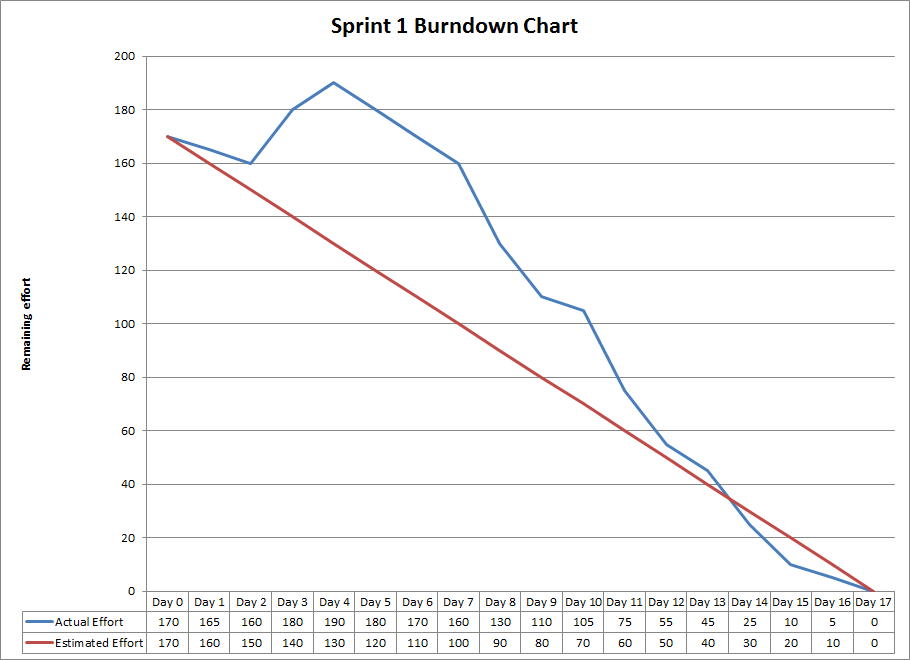
\includegraphics[width=1.0\textwidth]{burndown} % Include the image burndown.png
\end{center}
\end{figure}

\pagebreak

%individual sprint retrospective
\section{Individual Retrospective}
The following lists describe actions (as an individual) that will be started, stopped, or continued during the next sprint to maximize work efficiency. \\

Actions and/or items to \textbf{start} doing in the next sprint (top 3)
\begin{itemize}
\begin{item}
Description of first item
\end{item}
\begin{item}
Description of second item
\end{item}
\begin{item}
Description of third item
\end{item}
\end{itemize}

Actions and/or items to \textbf{stop} doing in the next sprint (top 3)
\begin{itemize}
\begin{item}
Description of first item
\end{item}
\begin{item}
Description of second item
\end{item}
\begin{item}
Description of third item
\end{item}
\end{itemize}

Actions and/or items to \textbf{continue} doing in the next sprint (top 3)
\begin{itemize}
\begin{item}
Description of first item
\end{item}
\begin{item}
Description of second item
\end{item}
\begin{item}
Description of third item
\end{item}
\end{itemize}

\end{document}